\section{Experiments}
\subsection{Setting}
% \paragraph{Implementation Details.}


\begin{table*}[t]
\small
\centering
% \setlength{\tabcolsep}{4pt}
\caption{Comparison of interactive part segmentation performance. We report IoU at different numbers of clicks, compared with Point-SAM~\cite{pointsam} and P3-SAM~\cite{p3sam} on PartObjaverse-Tiny~\cite{partobjaverse_tiny} and PartNeXT~\cite{partnext}.}
\label{tab:click_segmentation}
\begin{tabular}{l|ccccc ccccc}
\toprule
\multirow{2}{*}{Method}
& \multicolumn{5}{c}{PartObjaverse-Tiny}
& \multicolumn{5}{c}{PartNeXT} \\
\cmidrule(lr){2-6}\cmidrule(lr){7-11}
& IoU@1 & IoU@3 & IoU@5 & IoU@7 & IoU@10
& IoU@1 & IoU@3 & IoU@5 & IoU@7 & IoU@10 \\
\midrule
Point-SAM~\cite{pointsam} & 24.87 & 48.99 & 59.67 & 64.33 & 67.99 & 23.90 & 47.50 & 56.71 & 61.23 & 65.04 \\
P3-SAM~\cite{p3sam}       & 33.04 & 50.57 & 53.78 & 54.74 & 55.51 & 35.61 & 51.26 & 52.03 & 52.61 & 53.81 \\
\textbf{SegviGen}         & \textbf{42.49} & \textbf{61.14} & \textbf{67.53} & \textbf{71.50} & \textbf{75.02}
                          & \textbf{54.86} & \textbf{71.15} & \textbf{78.11} & \textbf{79.96} & \textbf{82.73} \\
\bottomrule
\end{tabular}
\end{table*}


\begin{figure*}[t]
  \centering
  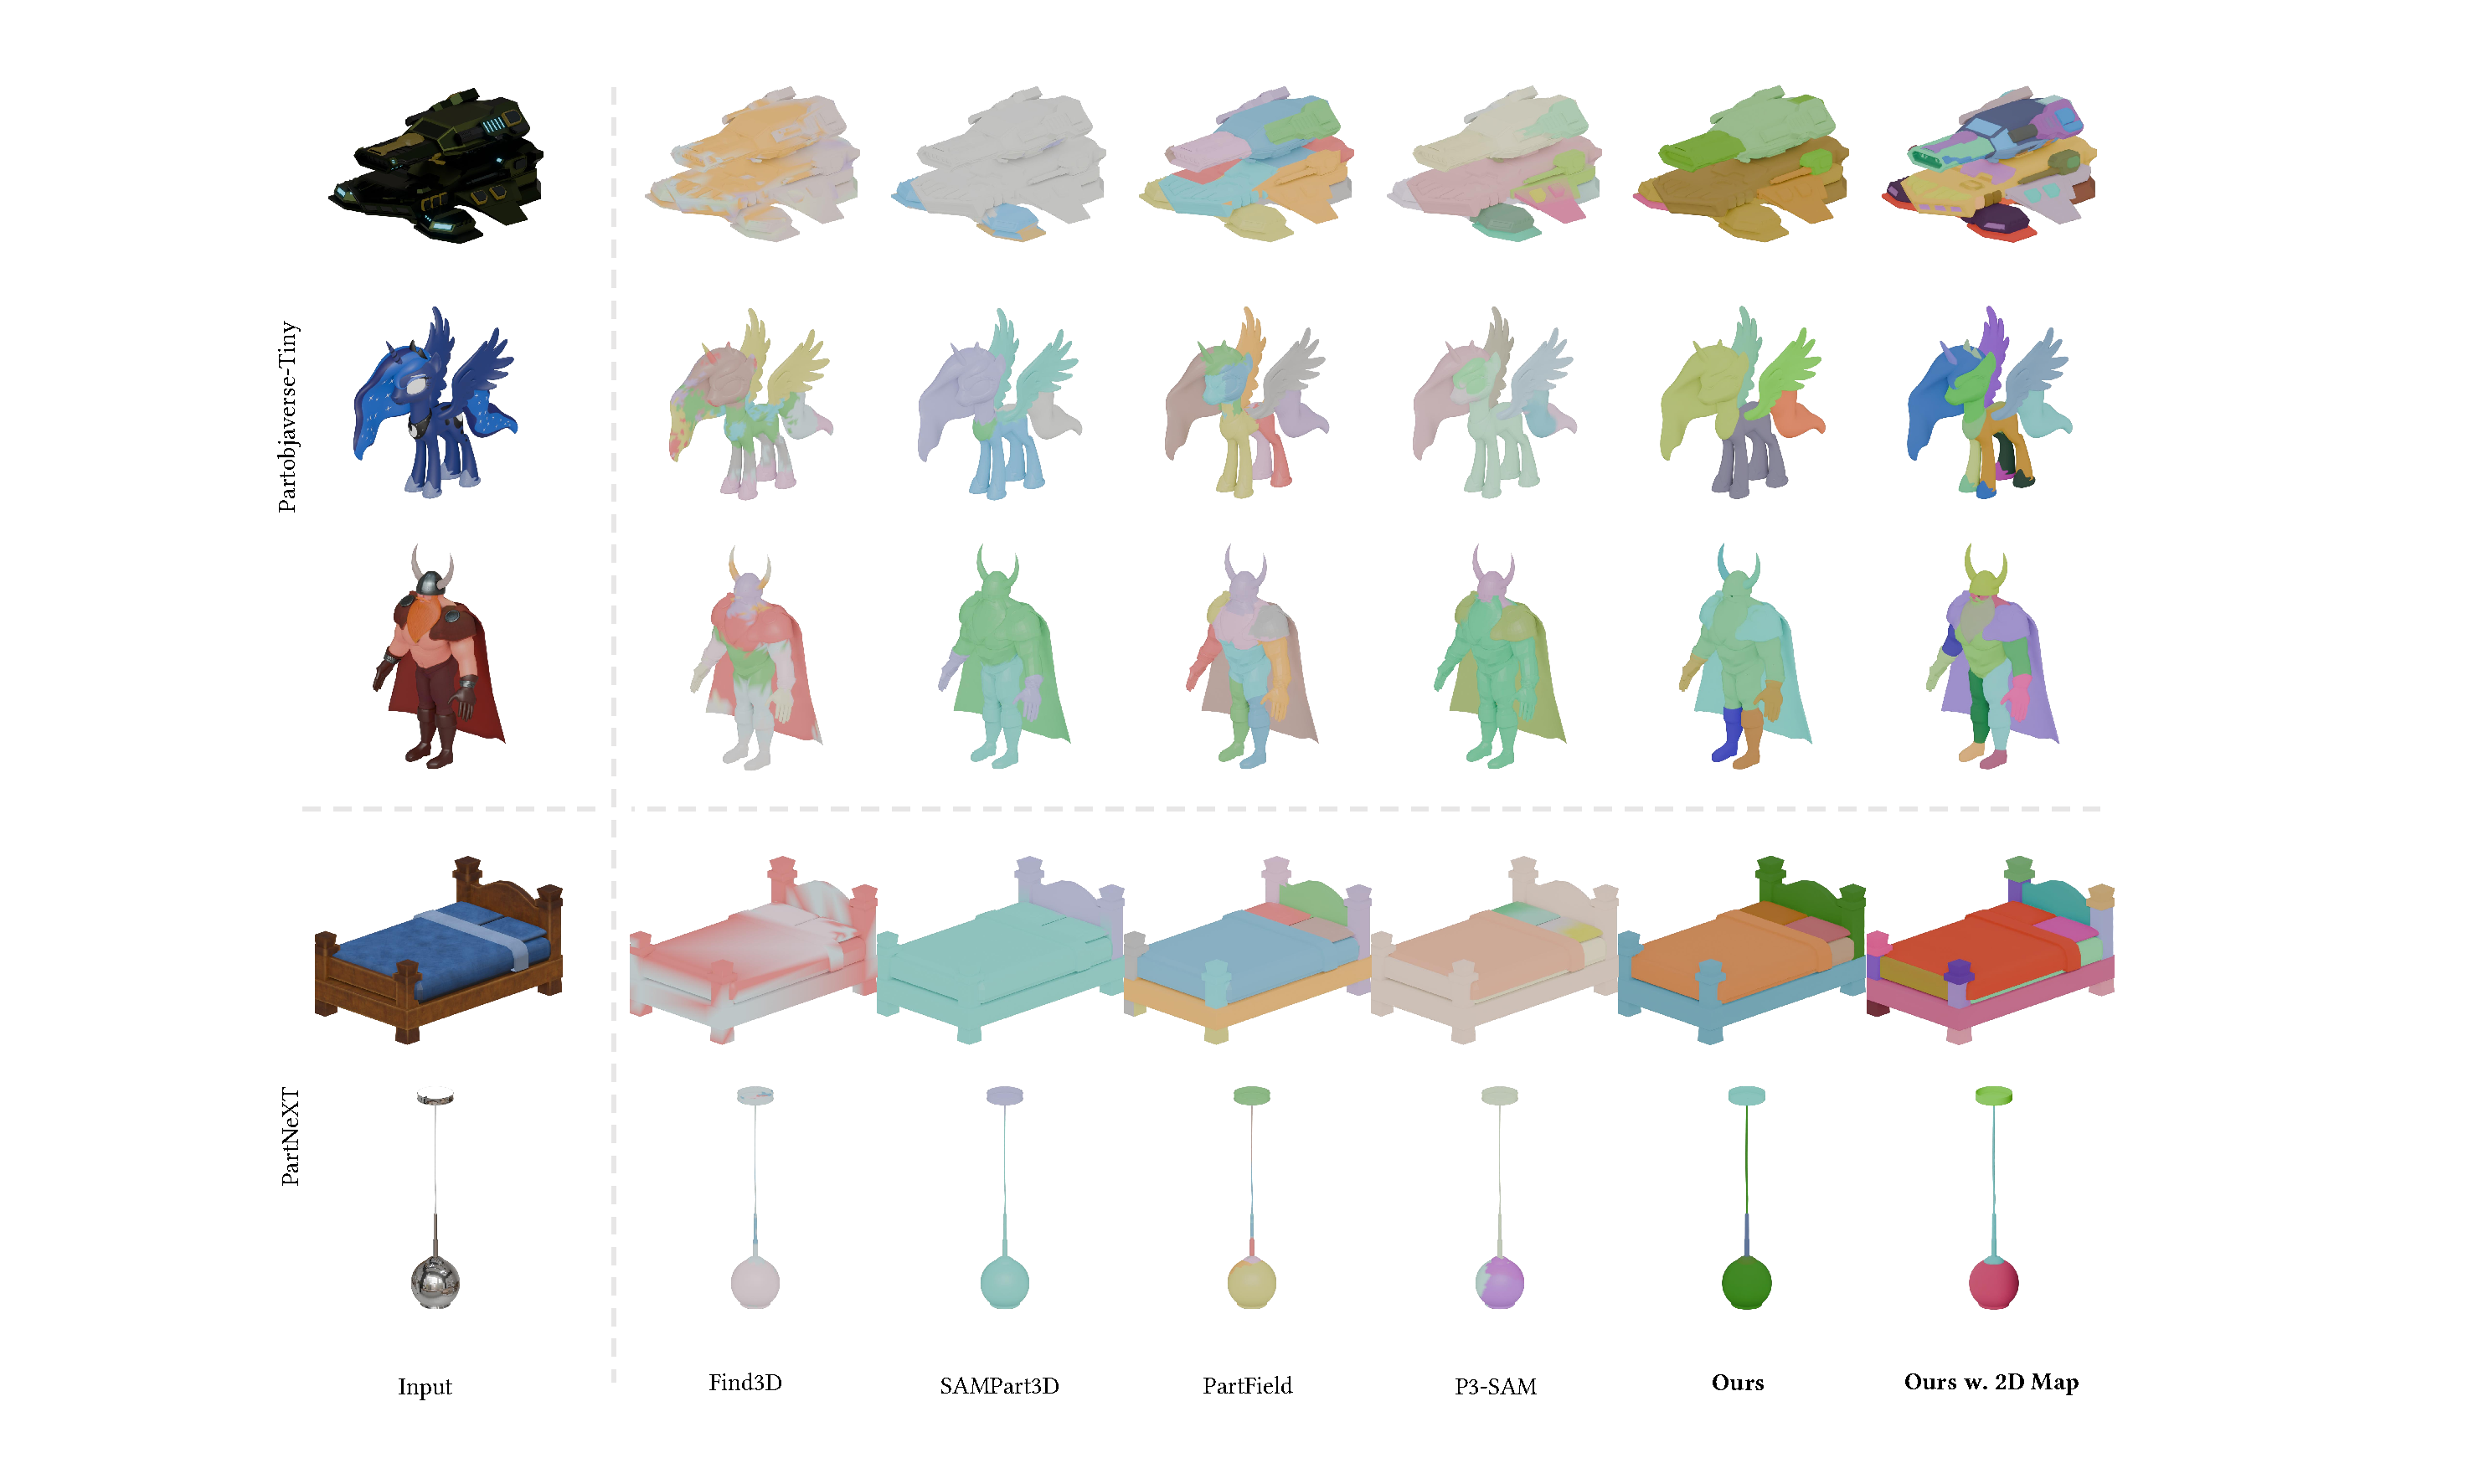
\includegraphics[width=\linewidth]{img/comparison_full.pdf}
  \caption{
    Full segmentation results. 
    %
    We compare \textit{SegviGen} against a broad set of prior methods, where different colors indicate different segmented parts. 
    %
    From the results, \textit{SegviGen} achieves high-accuracy full segmentation with sharp part boundaries using only 3D input. 
    %
    When 2D guidance is provided, it further allows explicit control over granularity and labels, enabling controllable, ultra-fine-grained 3D part parsing.
  }
  \label{fig:comparison_full}
\end{figure*}

\noindent \textbf{Implementation Details.}
%
We adopt Trellis.2~\cite{trellis2} as our base model, which is a 3D generative framework with a native and compact structured latent representation. 
%
For all experiments, the Tex-SLAT flow model is trainable, while the remaining SC-VAE is kept frozen.
%
We adopt the AdamW optimizer~\cite{adamw} with a learning rate of $1\times10^{-4}$. All experiments are conducted on 8 NVIDIA A800 GPUs, and the model is trained for  8 hours.
%
Unless otherwise specified, the segmentation results shown in this paper are produced with 12-step inference.

\noindent \textbf{Datasets.} % \paragraph{Datasets.}
For training, we use the PartVerse dataset~\cite{copartpartverse}, which contains 12k objects with a total of approximately 91k annotated parts.
%
For evaluation, we use PartObjaverse-Tiny~\cite{sampart3d}, which contains 200 textured mesh objects, and a 300-object textured-mesh subset of PartNeXT~\cite{partnext}.


\noindent \textbf{Baselines.}
We compared our model's performance on full segmentation between P3-SAM~\cite{p3sam}, Find3D~\cite{find3d}, SAMPart3D~\cite{sampart3d}, Partfield~\cite{partfield}.
P3-SAM is a native 3D point-promptable part segmenter with multiple mask heads and an IoU predictor. It can be run automatically by sampling prompt points and merging redundant masks with NMS.
Find3D targets open-world, language-queryable parts by auto-labeling rendered multi-view images with SAM and a VLM, projecting them back to 3D, and training a transformer to produce per-point features aligned to a CLIP-like embedding space for cosine-similarity querying.
SAMPart3D and PartField both learn part-aware 3D features from multi-view SAM masks and obtain parts via feature clustering.

For interactive part segmentation, we compared our model against P3-SAM~\cite{p3sam} and Point-SAM~\cite{pointsam}, where Point-SAM adapts the SAM prompt-and-mask paradigm to point clouds and is trained with SAM-generated pseudo masks.

\noindent \textbf{Metrics.}
To evaluate the interactive segmentation, we sample 10 positive points for each part, then measure the average IOU between the predicted masks for all clicks of all parts and their corresponding ground truth masks. \textbf{IoU@N} stands for IoU score in \textbf{N} foreground clicks.
The evaluation metric for full segmentation is the same method in previous work~\cite{p3sam,partfield}, using IoU to measure the accuracy of overall mask predictions. 
% 1. Setting

% 1.1 Implementation details
% 1.2 Baselines
% 1.3 Metrics
\subsection{Main Results}
\subsubsection{Interactive Part-Segmentation}

We evaluate interactive part segmentation on two benchmarks: PartObjaverse-Tiny~\cite{partobjaverse_tiny} and PartNeXT~\cite{partnext}.
%
We benchmark against two state-of-the-art native 3D methods: Point-SAM~\cite{pointsam}, which is specialized for point cloud segmentation, and P3-SAM~\cite{p3sam}. The quantitative results are summarized in Table~\ref{tab:click_segmentation}.

As shown in Table~\ref{tab:click_segmentation}, \textit{SegviGen} consistently outperforms all baselines by a significant margin across all interaction rounds. Notably, our method demonstrates exceptional efficiency in the \textit{few-shot} interaction setting. In the most challenging $1$-click scenario (IoU@1), \textit{SegviGen} achieves \textbf{42.49\%} on PartObjaverse-Tiny and \textbf{54.86\%} on PartNext, surpassing the Point-SAM by approximately \textbf{17.6\%} and \textbf{31.0\%}, respectively. This indicates that our generative framework possesses a much stronger initial understanding of 3D part structures compared to discriminative approaches, allowing it to infer complete part geometries from minimal user guidance.

Furthermore, as the number of user clicks increases from 1 to 10, \textit{SegviGen} exhibits a steady and robust performance gain. On the PartNext dataset, our method reaches an IoU of \textbf{82.73\%} at 10 clicks, significantly higher than Point-SAM (65.04\%) and P3-SAM (53.81\%). This demonstrates that our model effectively incorporates user feedback to refine boundaries and resolve ambiguities.

\subsubsection{Full Segmentation}

We evaluate the full segmentation capability of \textit{SegviGen} in two distinct settings:
(1) Using purely native 3D representation.
%
(2) Incorporating with 2D guidance. 
%
Quantitative comparisons with state-of-the-art methods, including Find3D~\cite{find3d}, SAMPart3D~\cite{sampart3d}, PartField~\cite{partfield}, and P3-SAM~\cite{p3sam}, are presented in Table~\ref{tab:auto_segmentation}.
Qualitative results are shown in \ref{fig:comparison_full}.

\noindent \textbf{Without 2D Guidance.}
In this setting, \textit{SegviGen} performs segmentation solely based on the structural and appearance priors learned during pretraining, without access to any external 2D segmentation maps. The model is prompted to generate part-indicative colors directly from the latent 3D representation.
As shown in Table~\ref{tab:auto_segmentation}, our method demonstrates superior generalization, particularly on PartNext. \textit{SegviGen} achieves an IoU of \textbf{55.40\%}, significantly outperforming PartField (41.50\%) and SAMPart3D (29.62\%)
While SAMPart3D performs well on the smaller PartObjaverse-Tiny dataset (59.05\%), its performance collapses on PartNext. In contrast, \textit{SegviGen} maintains robust performance (50.64\% on PartObjaverse-Tiny).

\noindent \textbf{With 2D Guidance.}
To further unleash the potential of \textit{SegviGen}, we introduce a 2D-guided mode where the model is conditioned on a single-view 2D segmentation map (rendered via nvdiffrast or derived from a 2D segmenter). This setting combines the rich semantic cues of 2D foundation models with the geometric consistency of our 3D generative framework.
Incorporating this lightweight 2D prior yields substantial performance gains. As shown in Table~\ref{tab:auto_segmentation}, \textit{SegviGen} (w. 2D Map) achieves new state-of-the-art results on both datasets, reaching \textbf{62.98\%} on PartObjaverse-Tiny and \textbf{71.53\%} on PartNext.



\begin{table}[t]
\small
  \centering
  \caption{Quantitative results (IoU) for full segmentation. “w. 2D Map” denotes the setting with 2D segmentation-map guidance.}
  \label{tab:auto_segmentation}
  % \setlength{\tabcolsep}{8pt}
  \begin{tabular}{l|rr}
    \toprule
    Method & PartObjaverse-Tiny & PartNext~ \\
    \midrule
    Find3D~\cite{find3d}            & 15.62 & 19.04 \\
    SAMPart3D~\cite{sampart3d}        & 59.05 & 29.62 \\
    PartField~\cite{partfield}       & 51.72 & 41.50 \\
    P3-SAM~\cite{p3sam}            & 45.36 & 31.94 \\
    \hline
    \textbf{SegviGen} & 50.64 & 55.40 \\
    \textbf{SegviGen (w. 2D Map)} & \textbf{62.98} & \textbf{71.53} \\
    \bottomrule
  \end{tabular}
\end{table}

\begin{figure*}
  \centering
  \includegraphics[width=0.92\linewidth]{img/more_results_ours.png}
  \caption{More qualitative segmentation results of our \textit{SegviGen}.}
  \label{fig:more_results_ours}
\end{figure*}

\begin{figure*}
  \centering
  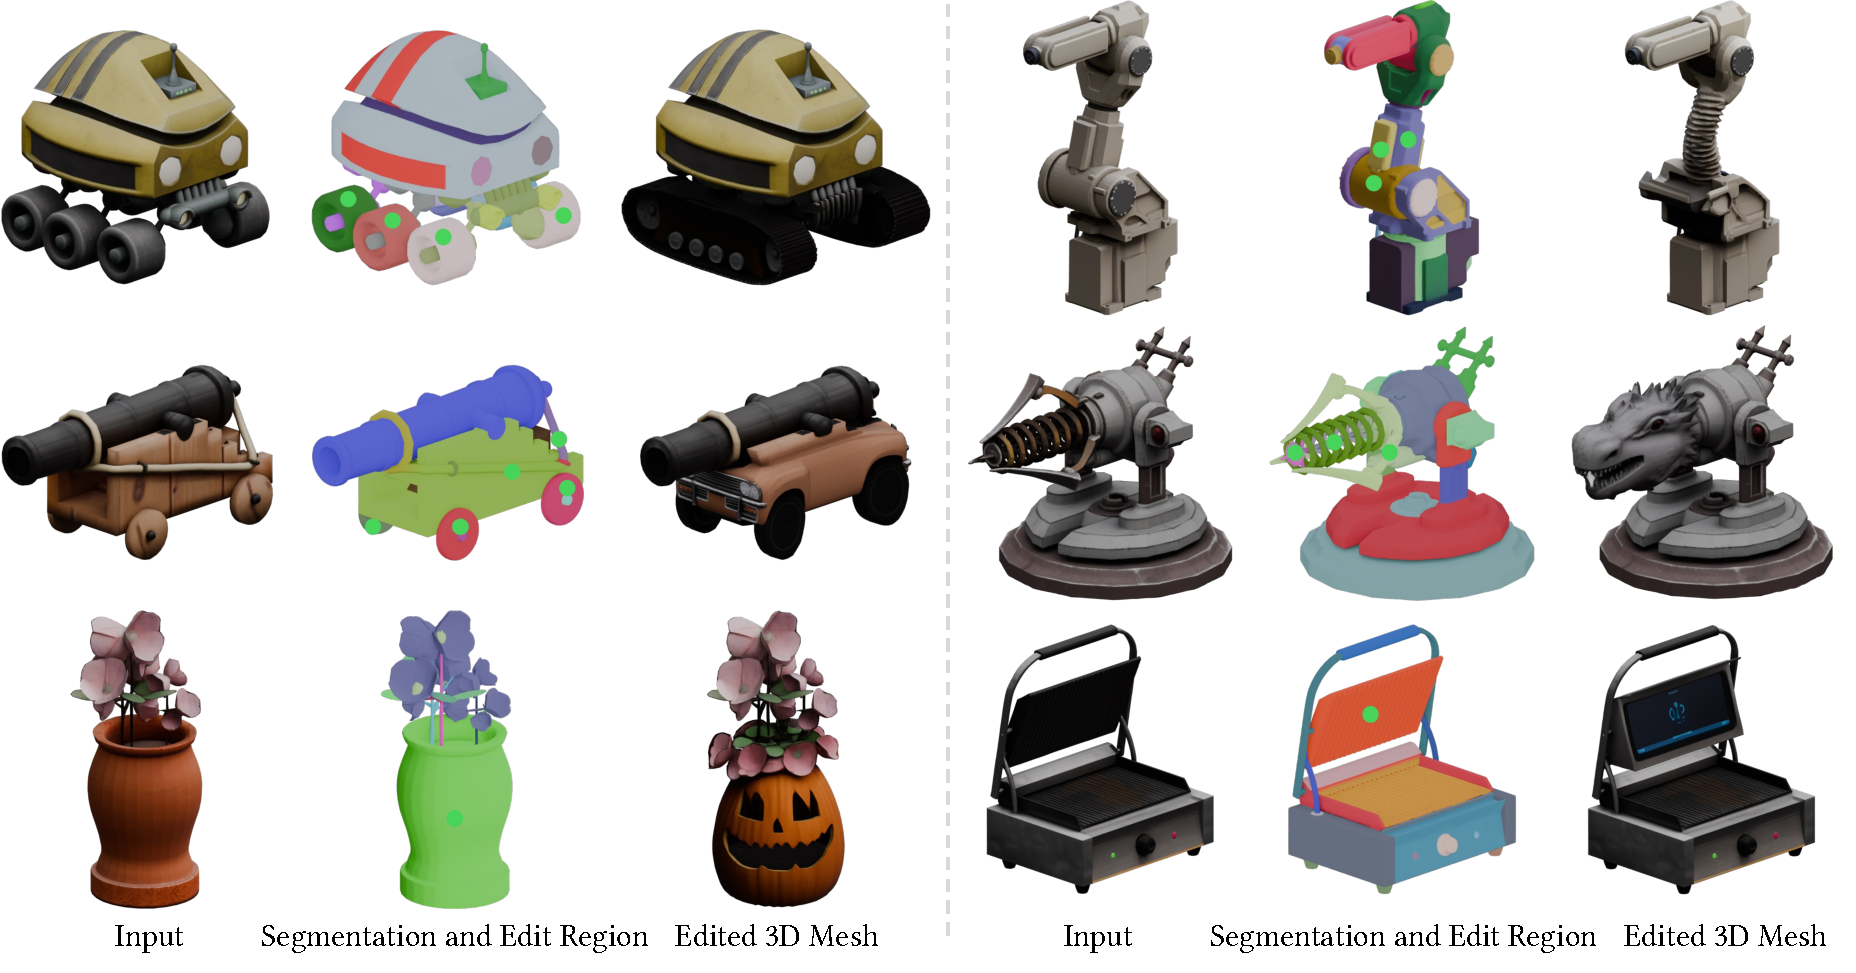
\includegraphics[width=0.92\linewidth]{img/more_apps_edit.pdf}
  \caption{
    Interactive 3D editing results with \textit{SegviGen} and \textit{VoxHammer}~\cite{voxhammer}.
    \textit{SegviGen} provides precise part segmentation to facilitate downstream editing models. 
    The target region to be edited is indicated by green points.
    It demonstrates the practical utility of \textit{SegviGen} in downstream 3D editing pipelines.
    }
  \label{fig:more_apps_edit}
\end{figure*}

% 表，图
\subsection{Ablation Studies and Analysis}
\subsubsection{Point Embedding Mechanism}
To investigate the optimal representation point prompt within our framework, we conducted an ablation study on the point embedding mechanism, comparing two distinct strategies:

\noindent \textbf{Explicit Coordinate Encoding.} 
In this setting, spatial coordinates are explicitly injected into the feature space. We utilize a frequency-based positional encoding scheme to map continuous 3D coordinates into high-dimensional embeddings, which will fuse with learnable semantic vectors. Consequently, the input features explicitly encapsulate both absolute spatial information and semantic category.

\noindent \textbf{Label-based Semantic Embedding.}
In this setting, the feature vectors serve solely as semantic indicators without explicitly encoding geometric values. A shared learnable embedding vector is assigned to all foreground points. The spatial information is preserved implicitly via the coordinate indices of the SparseTensor, relying on the sparse backbone's intrinsic ability to process spatial locality.

\begin{table}[t]
\small
  \centering
  \caption{Ablation study on point embedding mechanisms. We compare the performance of Explicit Coordinate Encoding and Label-based Semantic Embedding under varying numbers of clicks on PartObjaverse~\cite{partobjaverse_tiny}.}
  \label{tab:ablation_embedding}
  \setlength{\tabcolsep}{3.5pt}
  \begin{tabular}{l|ccccc}
    \toprule
    Method & IoU@1 & IoU@3 & IoU@5 & IoU@7 & IoU@10 \\
    \midrule
    Explicit Coord & 41.75 & 60.19 & 67.43 & 71.61 & 75.40 \\
    Label-based    & \textbf{42.49} & \textbf{61.14} & 67.53 & 71.50 & 75.02 \\
    \bottomrule
  \end{tabular}
\end{table}

\begin{table}[t]
\small
    \centering
    \caption{Effect of sampling steps on segmentation performance. We choose 12 steps as a practical trade-off between accuracy and efficiency.}
    \label{tab:steps_analysis}
    \setlength{\tabcolsep}{4pt}
    \begin{tabular}{l|cccccc}
    \toprule
    Steps & IoU@1 & IoU@3 & IoU@5 & IoU@7 & IoU@10 & Time \\
    \midrule
    1 & 42.90 & 59.98 & 65.86 & 69.50 & 72.85 & 0.44s \\
    4 & \textbf{44.51} & 60.40 & 66.65 & 70.64 & 73.58 & 1.02s \\
    8 & 44.21 & 61.14 & 67.64 & 71.14 & 74.49 & 1.81s \\
    12 & 42.49 & 61.14 & 67.53 & 71.50 & \textbf{75.02} & 2.63s \\
    25 & 43.82 & \textbf{61.67} & \textbf{68.30} & \textbf{71.87} & 74.99 & 5.12s \\
    \bottomrule
    \end{tabular}
\end{table}

Quantitative results demonstrate a distinct trend in the performance of point embedding mechanisms. As shown in Table \ref{tab:ablation_embedding}, the Label-based Semantic Embedding achieves slightly higher IoU scores when the number of clicks is limited (e.g., at 1 click). However, as the number of interactions increases, the Explicit Coordinate Encoding method consistently outperforms the Label-based approach, particularly in the later stages (e.g., 10 clicks).
We attribute this phenomenon to the nature of the embeddings: while label-based embeddings are sufficient for sparse guidance, explicit positional encodings provide a finer granularity of spatial differentiation. This capability becomes increasingly critical when processing a larger set of points, allowing the model to better resolve complex geometric details from multiple user constraints.


% 3.1 Point embedding 机制

\subsubsection{Number of Denoising Steps at Inference}

We analyze the impact of sampling steps on segmentation performance in Table \ref{tab:steps_analysis}. Due to the trajectory property of the flow model, we observe a great performance even with one step. Performance improves as steps increase, but gains begin to saturate over 8 steps. Although 25 steps offer marginal improvements, the inference latency nearly doubles compared to 12 steps. Thus we adopt 12 steps as the optimal balance between high-quality results and computational efficiency.

